\documentclass[border=10pt]{standalone}
\usepackage{tikz}
\usetikzlibrary{arrows.meta, shapes, calc}
\usepackage{amsmath}
\begin{document}
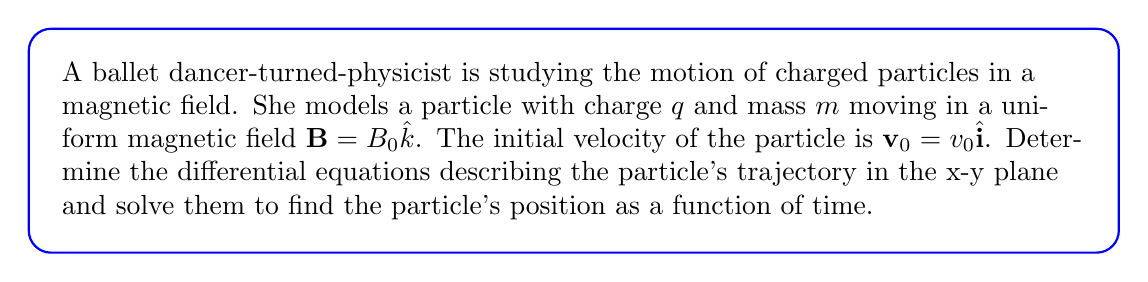
\begin{tikzpicture}
\node (problem) [
    draw=blue,
    thick,
    rounded corners=8pt,
    inner sep=12pt,
    text width=13cm,
    align=left,
    font=\normalsize
] {
A ballet dancer-turned-physicist is studying the motion of charged particles in a magnetic field. She models a particle with charge $q$ and mass $m$ moving in a uniform magnetic field $\mathbf{B} = B_0 \hat{k}$. The initial velocity of the particle is $\mathbf{v}_0 = v_0 \hat{\mathbf{i}}$. Determine the differential equations describing the particle's trajectory in the x-y plane and solve them to find the particle's position as a function of time.
};
\end{tikzpicture}
\end{document}